\chapter{Arhitektura i dizajn sustava}
Arhitektura se može podijeliti na tri podsustava:
\begin{packed_item}
	\item web poslužitelj
	\item web aplikacija
	\item baza podataka
\end{packed_item}
\underbar{Web preglednik} je program koji korisniku omogućuje pregled web-stranica i multimedijalnih sadržaja vezanih uz njih. Svaka stranica pisana je u kodu, a web preglednik je pretvara u ono što mi vidimo. Dakle, svaki internetski preglednik je
prevoditelj. Korisnik putem web preglednika šalje zahtjev web poslužitelju.
\newline \underbar{Web poslužitelj} osnova je rada web aplikacije. On šalje i prima podatke od mnogostrukih klijenata. Komunikacija između njega i korisnika se odvija preko HTTP (engl. Hyper Text Transfer Protocol) protokola, što je protokol u prijenosu informacija na webu. Poslužitelj je onaj koji pokreće web aplikaciju te joj prosljeđuje
zahtjev.
\newline Za obrađivanje željenih zahtjeva koristi se \underbar{web aplikacija}. Ako je potrebno pristupa
bazi podataka te preko poslužitelja korisniku vraća odgovor u obliku HTML dokumenta vidljivog u web pregledniku.
\newline Programski jezik koji smo odabrali za izradu naše web aplikacije je JavaScript zajedno
sa Bootstrap radnim okvirom te HTML i CSS programske jezike za oblikovanje.
Odabrano razvojno okruženje programske potpore je Visual studio code.
\newline Temelj arhitekture sustava ležat će na MVC (Model-View-Controller) konceptu. Naime, taj koncept ima već napravljene predloške koji nam pomažu u izradi web aplikacije te je podržan od radnog okvira. Velika prednost MVC koncepta je da omogućuje programeru da razvija komponente aplikacije nezavisno jedne o drugima,
što olakšava testiranje, traženje grešaka i dodavanje novih funkcionalnosti.
\newline MVC koncept sastoji se od 3 dijela:
\begin{packed_item}
	\item Model – centralni dio sustava koji direktno upravlja podacima, logikom i pravilima sustava. Isto tako prima ulazne podatke Controllera
	\item View – glavna uloga mu je da prikazuje podatke. Ista informacija može se prikazati na nekoliko različitih načina, poput grafova, tablica i sl.
	\item Controller – bavi se prilagodavanjem ulaza koje prosljeduje Modelu i Viewu te upravlja zahtjevima korisnika i pomoću njih djeluje na ostale sustave.
\end{packed_item}

		
		\section{Baza podataka}
			
Za potrebe našeg sustava za organizaciju kampa računarstva „Mlade nade” koristimo relacijsku bazu podataka. Relacijska baza sastoji se od relacija, tj. tablica koje sadrže naziv i skup atributa. Ovakva baza nam omogućuje brzu i jednostavnu pohranu i izmjenu podataka te dohvat podataka za daljnju obradu. Dijagram baze olakšava razumijevanje namjene podataka i njihove povezanosti.\\
Baza podataka ove aplikacije sastoji se od sljedećih entiteta:
\begin{packed_item}
	\item Osoba
	\begin{packed_item}
		\item Animator
		\item Sudionik
		\item Organizator
	\end{packed_item}
	\item Aktivnost
	\begin{packed_item}
		\item Aktivnost1
		\item AktivnostSve
		\item AktivnostMaxN
		\item AktivnostN
	\end{packed_item}
	\item Grupa
	\item Sudjeluje
	\item Račun
	\item Dojam
	\item Prijava
	\item Kamp
\end{packed_item} 
\subsection {Opis tablica}
\textit {\textbf{osoba -}} ovaj entitet sadrži podatke o osobama koje na bilo koji način sudjeluju u kampu. Sadrži atribute: puno ime osobe, ID osobe, motivacijsko pismo, datum rođenja, broj telefona odgovorne osobe (za sudionike mlađe od 18 godina), e-mail i broj telefona. Generalizacija je entiteta organizator, animator i sudionik. U vezi je one-to-one s entitetom dojam preko atributa Idosobe.
\\
\definecolor{aquamarine}{rgb}{0.5, 1.0, 0.83}
\definecolor{blizzardblue}{rgb}{0.67, 0.9, 0.93}
\begin{tabular} {|l|l|l|}
	
	\hline \multicolumn{3}{|c|}{\textbf{osoba}}	 \\ \hline
	
	\cellcolor{aquamarine}Idosobe & INT	&  	identifikacijski broj osobe\\ \hline
	punoIme	& VARCHAR &   ime i prezime osobe	\\ \hline 
	motPismo & VARCHAR &  motivacijsko pismo \\ \hline 
	datumRod & DATE	&  	datum rođenja osobe	\\ \hline 
	brojTelefonaOdgOsobe & 	VARCHAR	&	broj telefona odgovorne osobe \\ \hline
	Email &	VARCHAR	&	e-mail osobe \\ \hline
	brojTel	&	VARCHAR	&	broj telefona osobe \\ \hline
\end{tabular}\\
\\
\\
\textbf{\textit{animator -}} ovaj entitet sadrži podatke o animatorima koji sudjeluju u raznim aktivnostima. Specijalizacija je entiteta osoba. Uz atribute entiteta osoba sadrži još i entitet naziv aktivnosti. U vezi je many-to-one s entitetom aktivnost preko atributa nazivAkt.\\
\begin{tabular}{|l|l|l|}
	
	\hline \multicolumn{3}{|c|}{\textbf{animator}}	\\  \hline
	
	\cellcolor{aquamarine}Idosobe & INT	&  	identifikacijski broj osobe\\ \hline
	\cellcolor{blizzardblue}nazivAkt	& VARCHAR &   naziv aktivnosti u kojoj sudjeluje	\\ \hline 
	punoIme	& VARCHAR &   ime i prezime osobe	\\ \hline 
	motPismo & VARCHAR &  motivacijsko pismo \\ \hline 
	datumRod & DATE	&  	datum rođenja osobe	\\ \hline 
	brojTelefonaOdgOsobe & 	VARCHAR	&	broj telefona odgovorne osobe \\ \hline
	Email &	VARCHAR	&	e-mail osobe \\ \hline
	brojTel	&	VARCHAR	&	broj telefona osobe \\ \hline
\end{tabular} \\ \\
\\
\\
\textbf{\textit{sudionik -}} ovaj entitet sadrži podatke o sudionicima kampa. Specijalizacija je entiteta osoba. Uz atribute entiteta osoba sadrži još i entitet naziv grupe. U vezi je many-to-one s entitetom grupa preko atributa nazivGrupa.\\
\begin{tabular}{|l|l|l|}
	
	\hline \multicolumn{3}{|c|}{\textbf{Sudionik}}\\ \hline
	
	\cellcolor{aquamarine}Idosobe & INT	&  	identifikacijski broj osobe\\ \hline
	\cellcolor{blizzardblue}nazivGrupa	& VARCHAR &   naziv grupe čiji je član	\\ \hline 
	punoIme	& VARCHAR &   ime i prezime osobe	\\ \hline 
	motPismo & VARCHAR &  motivacijsko pismo \\ \hline 
	datumRod & DATE	&  	datum rođenja osobe	\\ \hline 
	brojTelefonaOdgOsobe & 	VARCHAR	&	broj telefona odgovorne osobe \\ \hline
	Email &	VARCHAR	&	e-mail osobe \\ \hline
	brojTel	&	VARCHAR	&	broj telefona osobe \\ \hline
\end{tabular} \\ \\
\\
\textbf{\textit{organizator -}} ovaj entitet sadrži informacije o osobi koja organizira kamp. Specijalizacija je entiteta osoba. Uz atribute entiteta osoba sadrži još i entitet nazivGrupa.\\
\begin{tabular}{|l|l|l|}
	
	\hline \multicolumn{3}{|c|}{\textbf{organizator}}\\	 \hline
	
	\cellcolor{aquamarine}Idorganizatora & INT	&  	identifikacijski broj organizatora\\ \hline
	punoIme	& VARCHAR &   ime i prezime osobe	\\ \hline 
	motPismo & VARCHAR &  motivacijsko pismo \\ \hline 
	datumRod & DATE	&  	datum rođenja osobe	\\ \hline 
	brojTelefonaOdgOsobe & 	VARCHAR	&	broj telefona odgovorne osobe \\ \hline
	Email &	VARCHAR	&	e-mail osobe \\ \hline
	brojTel	&	VARCHAR	&	broj telefona osobe \\ \hline 
\end{tabular} \\ \\
\\
\textbf{\textit{aktivnost -}} ovaj entitet sadrži podatke o aktivnostima koje se odvijaju u kampu. Generalizacija je entiteta aktivnost1, aktivnostSve, aktivnostMaxN i aktivnostN. Sadrži atribute naziv aktivnosti, opis i trajanje aktivnosti. U vezi je many-to-one s entitetom sudjeluje preko atributa nazivAkt. \\
\begin{tabular}{|l|l|l|}
	
	\hline \multicolumn{3}{|c|}{\textbf{aktivnost}}	\\ \hline
	
	\cellcolor{aquamarine}nazivAkt & VARCHAR &  Naziv aktivnosti\\ \hline 
	opis &	VARCHAR	& Kratak opis aktivnosti\\ \hline
	trajanje & INTERVAL & Trajanje aktivnosti\\ \hline
\end{tabular} \\ \\
\\
\textbf{\textit{aktivnost1 -}} ovaj entitet sadrži podatke o aktivnostima u kojima sudjeluje samo jedna grupa sudionika. Specijalizacija je entiteta aktivnost. Sadrži sve atribute entiteta aktivnost tj. naziv aktivnosti, opis i trajanje.\\
\begin{tabular}{|l|l|l|l|}
	
	\hline \multicolumn{3}{|c|}{\textbf{aktivnost1}}\\ \hline
	
	\cellcolor{aquamarine}nazivAkt & VARCHAR	&  	naziv aktivnosti\\ \hline 
	opis	&	VARCHAR	&	kratak opis aktivnosti\\ \hline
	trajanje & INTERVAL & trajanje aktivnosti\\ \hline
\end{tabular} \\ \\
\\
\textit{\textbf{aktivnostSve -}} ovaj entitet sadrži podatke o aktivnostima u kojima sudjeluju sve postojeće grupe sudionika. Specijalizacija je entiteta aktivnost. Sadrži sve atribute entiteta aktivnost tj. naziv aktivnosti opis i trajanje.\\
\begin{tabular}{|l|l|l|l|}
	
	\hline \multicolumn{3}{|c|}{\textbf{aktivnostSve}}	\\  \hline
	
	\cellcolor{aquamarine}nazivAkt & VARCHAR	&  	naziv aktivnosti\\ \hline 
	opis	&	VARCHAR	&	kratak opis aktivnosti\\ \hline
	trajanje & INTERVAL & trajanje aktivnosti\\ \hline
\end{tabular} \\ \\
\\
\textbf{\textit{aktivnostMaxN -}} ovaj entitet sadrži podatke o aktivnostima u kojima sudjeluje maksimalno N grupa sudionika. Specijalizacija je entiteta aktivnost. Sadrži sve atribute entiteta aktivnost tj. naziv aktivnosti, opis i trajanje.\\
\begin{tabular}{|l|l|l|l|}
	
	\hline \multicolumn{3}{|c|}{\textbf{aktivnostMaxN}}	\\  \hline
	
	\cellcolor{aquamarine}nazivAkt & VARCHAR	&  	naziv aktivnosti\\ \hline
	opis	&	VARCHAR	&	kratak opis aktivnosti\\ \hline
	trajanje & INTERVAL & trajanje aktivnosti\\ \hline 
\end{tabular} \\ \\
\\
\textbf{\textit{aktivnostN -}} ovaj entitet  sadrži podatke o aktivnostima u kojima sudjeluje točno N grupa sudionika. Specijalizacija je entiteta aktivnost. Sadrži sve atribute entiteta aktivnost tj. naziv aktivnosti, opis i trajanje.\\
\begin{tabular}{|l|l|l|l|}
	
	\hline \multicolumn{3}{|c|}{\textbf{aktivnostN}}\\	 \hline
	
	\cellcolor{aquamarine}nazivAkt & VARCHAR	&  	naziv aktivnosti\\ \hline
	opis	&	VARCHAR	&	kratak opis aktivnosti\\ \hline
	trajanje & INTERVAL & trajanje aktivnosti\\ \hline 
\end{tabular} \\ \\
\\
\textbf{\textit{grupa -}} ovaj entitet opisuje grupe sudionika koji sudjeluju u aktivnostima. Sadrži atribut naziv grupe. U vezi je many-to-one s entitetom sudjeluje preko atributa nazivGrupa. \\
\begin{tabular}{|l|l|l|l|}
	
	\hline \multicolumn{3}{|c|}{\textbf{grupa}}	\\  \hline
	
	\cellcolor{aquamarine}nazivGrupa & VARCHAR	&  	naziv grupe sudionika\\ \hline 
\end{tabular} \\ \\
\\
\textbf{\textit{sudjeluje -}} ovaj entitet sadrži sve informacije o odnosu grupa i aktivnosti, odnosno daje informacije o tome koja grupa sudjeluje u kojoj od aktivnosti. Sadrži atribut naziv grupe te je preko tog atributa u vezi one-to-many s entitetom sudionik.\\
\begin{tabular}{|l|l|l|l|}
	
	\hline \multicolumn{3}{|c|}{\textbf{sudjeluje}}\\	  \hline
	
	\cellcolor{aquamarine}nazivGrupa & VARCHAR	&  	naziv grupe sudionika\\ \hline 
	\cellcolor{aquamarine} nazivAkt	&	VARCHAR	&	naziv aktivnosti\\ \hline
\end{tabular} \\ \\
\\
\textbf{\textit{račun -}} ovaj entitet sadrži podatke o korisničkom računu koji je se izrađuje na temelju prihvaćene prijave za svakog sudionika i animatora. Sadrži atribute korisnickoIme, lozinka, poveznica i Idosobe. U vezi je one-to-one s entitetom osoba preko atributa Idosobe. \\
\begin{tabular}{|l|l|l|l|}
	
	\hline \multicolumn{3}{|c|}{\textbf{račun}}	\\  \hline
	
	\cellcolor{aquamarine}korisnickoIme & VARCHAR	&  	korisničko ime osobe\\ \hline 
	\cellcolor{blizzardblue} Idosobe	&	INT	&	identifikacijski broj osobe\\ \hline
	lozinka	&	VARCHAR	&	lozinka korisničkog računa\\ \hline
	poveznica	&	VARCHAR	&	poveznica za registraciju\\ \hline
\end{tabular} \\ \\
\\
\textbf{\textit{dojam -}} ovaj entitet sadrži informacije o osvrtu i ocjeni koju sudionici i animatori ostavljaju nakon završetka kampa. Sadrži entitete ID osobe, ocjena, komentar. U vezi je one-to-one s entitetom osoba preko atributa Idosobe.\\
\begin{tabular}{|l|l|l|l|}
	
	\hline \multicolumn{3}{|c|}{\textbf{dojam}}	\\  \hline
	
	\cellcolor{aquamarine}Idosobe	&	INT	&	identifikacijski broj osobe\\ \hline
	ocjena	&	INT	&	ocjena kampa\\ \hline
	komentar	&	VARCHAR	&	kratki osvrt\\ \hline
\end{tabular} \\ \\
\\
\textbf{\textit{prijava -}} ovaj entitet sadrži podatke o prijavama za sudjelovanje u kampu. Sadrži atribute prijavaZa (određuje prijavljuje li se osoba za sudionika ili animatora), vrijeme početka prijave i vrijeme trajanja prijave. \\
\begin{tabular}{|l|l|l|l|}
	
	\hline \multicolumn{3}{|c|}{\textbf{prijava}}\\	\hline
	
	prijavaZa	&	VARCHAR	&	prijava za sudionika/animatora\\ \hline
	vrijemePocetka	&	TIMESTAMP	&	vrijeme početka prijave\\ \hline
	vrijemeTrajanja	&	INTERVAL	&	trajanje prijave\\ \hline
\end{tabular} \\ \\
\\
\textbf{\textit{kamp -}} ovaj enitet sadrži informacije o kampu za računarstvo za koji se izrađuje aplikacija. Sadrži atribute vrijemePocetka i vrijemeTrajanje.\\
\begin{tabular}{|l|l|l|l|}
	
	\hline \multicolumn{3}{|c|}{\textbf{kamp}}\\	  \hline
	
	vrijemePocetka	&	TIMESTAMP	&	vrijeme početka kampa\\ \hline
	vrijemeTrajanja	&	INTERVAL	&	trajanje kampa\\ \hline
\end{tabular} \\ \\


			
			
			\subsection{Dijagram baze podataka}
\vspace {10pt} \textbf {Dijagram baze podataka}\\
\begin{figure}[htb]
	\centering
	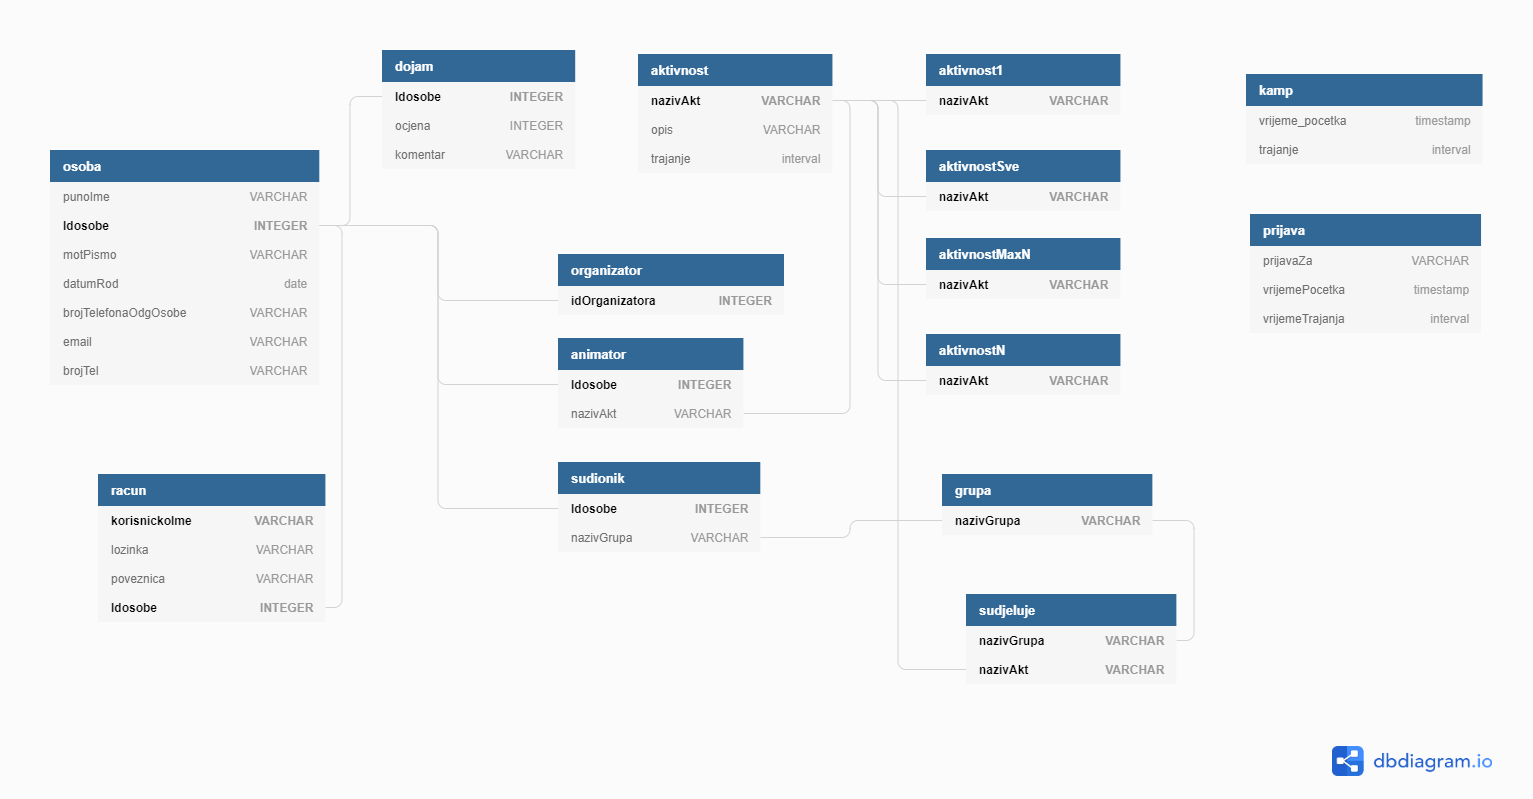
\includegraphics[scale=0.25]{dijagrami/dataBase.PNG}
	\caption{ER dijagram baze podataka}
	\label{fig: dijagram baze}
\end{figure}
			
			\eject
			
			\newpage
			
		\section{Dijagram razreda}
		
Na slikama 4.2 i 4.3 prikazani su razredi koji pripadaju backend dijelu MVCarhitekture.  Razredi prikazani na slici 4.2 nasljeduju Controller razred.  Metode implementirane u tim razredima manipuliraju s podacima, a oni su dohvaćeni pomoću metoda implementiranih u Model razredima.  Metode implementirane u Controller razredima vraćaju JSON datoteke s html status kodom. Prikazane su samo ovisnosti između razreda koji pripadaju istom dijelu dijagrama. Iz naziva i tipova atributa u razredima možemo zaključiti vrstu ovisnosti među različitim razredima. \\
\begin{figure}[htpb]
	\centering
	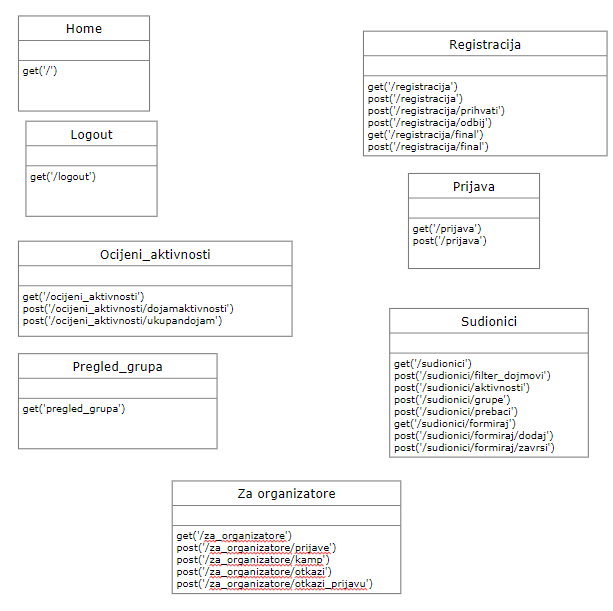
\includegraphics[scale=1]{dijagrami/controller_uml.PNG}
	\caption{Dijagram razreda - dio Controllers}
	\label{fig: dijagram razreda models}
\end{figure}
\newpage

Model razredi preslikavaju strukturu baze podataka u aplikaciji. Metode koje su implementirane direktno komuniciraju s bazom podataka i tako vraćaju tražene podatke. Razred Korisnik predstavlja neregistriranog korisnika koji se može registrirati u sustav unoseći tražene informacije. Također ako je već registriran, može se prijaviti u sustav. Nakon prijave on može biti registriran kao Sudionik ili kao Animator, i ovisno o tome može koristiti drugačije funkcionalnosti stranice. Razred Organizator predstavlja osobu koja može razmještati ostale korisnike po grupama i koja ima najveće ovlasti.\\

\begin{figure}[htpb]
	\centering
	\includegraphics[scale=0.3]{dijagrami/UMLdiagram.PNG}
	\caption{Dijagram razreda - dio Models}
	\label{fig: dijagram razreda models}
\end{figure}
\eject

		\eject
		\newpage
		
		\section{Dijagram stanja}
			
			
Dijagram stanja je dijagram koji prikazuje određena stanja objekata i prijelaze jednog stanja u drugo temeljene na određenim događajima. Na slici 4.4 prikazan je dijagram stanja za prijavu otprije registriranog korisnika – Sudionika i o prikazu njegovih opcija ovisno o tome je li kamp počeo, traje, ili je završio. Nakon prijave, ako kamp još nije počeo sudioniku se prikazuje odbrojavanje do početka kampa i klikom može kontaktirati organizatora. Nakon prijave i nakon početka kampa, sudionik vidi svoj osobni raspored ili agendu, te klikom na \textit{Popis članova} može vidjeti popis članova i njihove kontakte. Naposljetku, nakon prijave i nakon završetka kampa, sudionik može ocijeniti svoje cjelokupno iskustvo i ostaviti dojam.
			
\begin{figure}[htb]
	\centering
	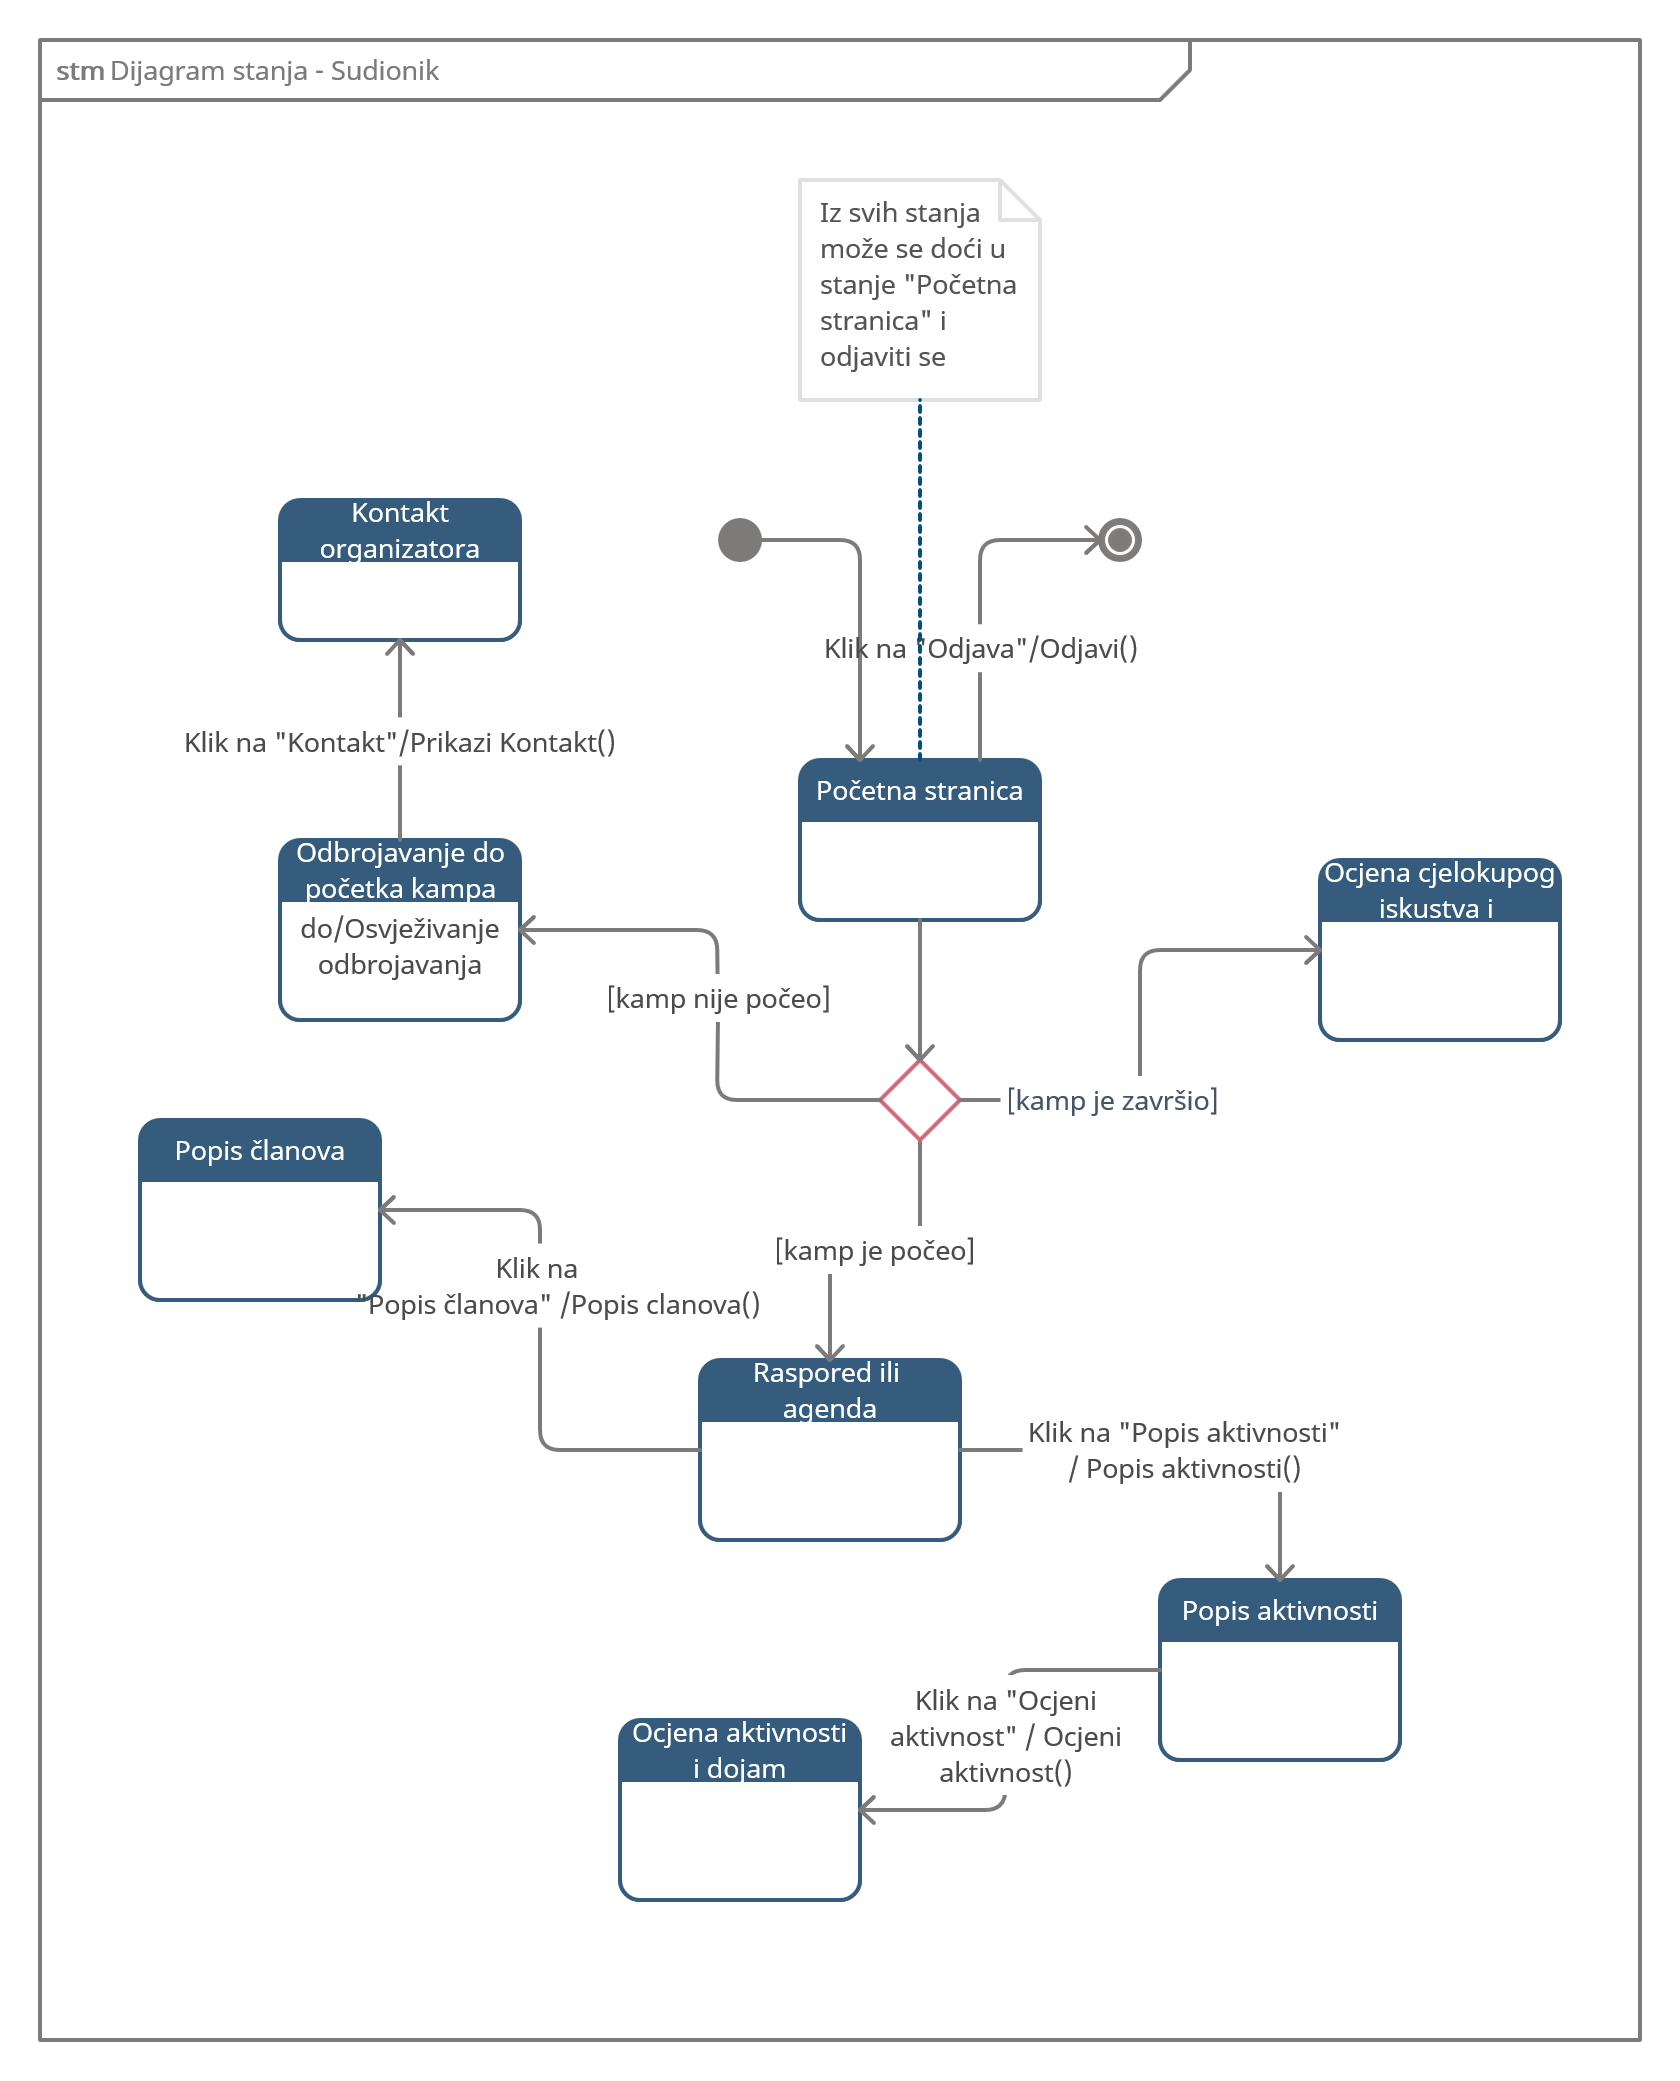
\includegraphics[scale=0.2]{dijagrami/dijagramStanja.PNG}
	\caption{Dijagram stanja}
	\label{fig: dijagram stanja}
\end{figure}
		\eject
		
		\section{Dijagram aktivnosti}
			
Dijagram aktivnosti primjenjuje se za opis modela toka upravljanja ili podatkovnog toka te modeliranje poslovnih procesa. To je u osnovi dijagram toka koji predstavlja tok iz jedne u drugu aktivnost. U modeliranju toka upravljanja svaki novi korak poduzima se nakon završenog prethodnog, a naglasak je na jednostavnosti.
Na slici 4.5 prikazan je proces ostavljanje dojma i ocjene korisnika za određenu aktivnost. Korisnik se prijavi u sustav te s popisa odabere jednu od aktivnosti u kojima sudjeluje. Zatim mu se prikazuje okvir za upis dojma i ocjene. Nakon upisivanja dojma i ocjene, podaci se spremaju u bazu podataka i korisnik se može odjaviti. \\

\begin{figure}[htb]
	\centering
	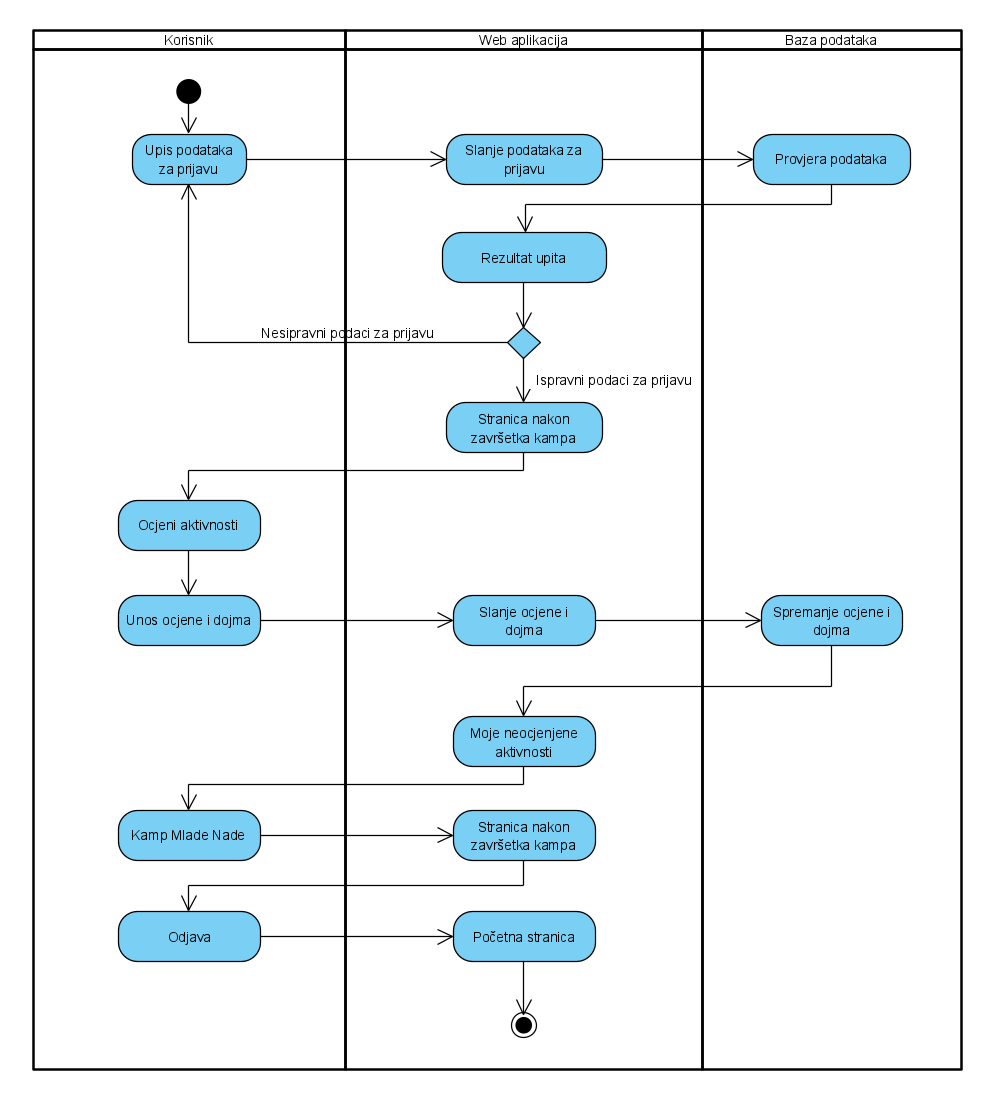
\includegraphics[scale=0.5]{dijagrami/dijagramAktivnosti.PNG}
	\caption{Dijagram aktivnosti}
	\label{fig: dijagram aktivnosti}
\end{figure}

		\eject
		
	\section{Dijagram komponenti}
	
		Sustavu se pristupa putem dva sučelja. Preko sučelja za dohvat HTML, CSS i JS datoteka poslužuju se datoteke koje pripadaju frontendu. Router je komponenta koja na upit s url-om određuje koja će se datoteka poslužiti na sučelje. Frontend se sastoji od niza JavaScript datoteka koje su raspoređene u simboličke cjeline i ovise o React biblioteci iz koje dohvaćaju gotove komponente (gumbi, forme i sl.). Backend je baziran na arhitekturi \textit{Repository Service Controller}. Preko
		sučelja za dohvat JSON podataka pristupa se REST API komponenti. REST API poslužuje podatke koji pripadaju backendu. Razredi koji implementiraju sučelje Service zaduženi su za dohvaćanje podataka iz baze podataka pomoću SQL upita uz pomoć Repositoryja. Podaci koji su pristigli iz baze šalju se MVC arhitekturi u obliku DTO (Data transfer object). React-view komponenta preko dostupnih sučelja komunicira s web aplikacijom te osvježava prikaz i dohvaća nove podatke.
		\begin{figure}[htb]
			\centering
			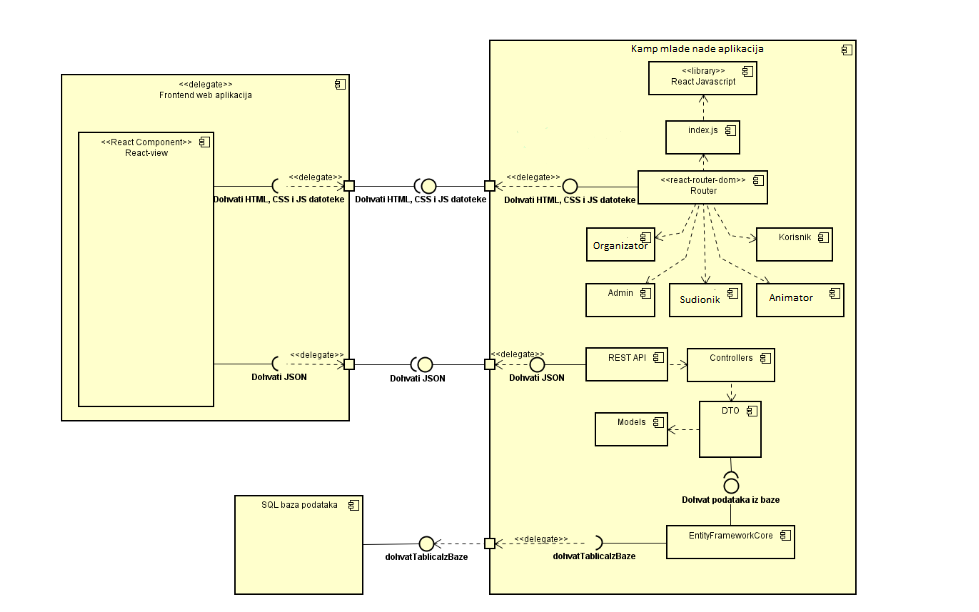
\includegraphics[scale=0.54]{dijagrami/dijagramKomponenti.PNG}
			\caption{Dijagram komponenti}
			\label{fig: dijagram komponenti}
		\end{figure}
			\eject